\documentclass{article}%
\usepackage[T1]{fontenc}%
\usepackage[utf8]{inputenc}%
\usepackage{lmodern}%
\usepackage{textcomp}%
\usepackage{lastpage}%
\usepackage{geometry}%
\geometry{margin=1in}%
\usepackage[utf8]{inputenc}%
\usepackage[titletoc,title]{appendix}%
\usepackage{graphicx,float}%
\usepackage{ragged2e}%
%
\title{\textbf{RELATÓRIO TÉCNICO DE SAÚDE PÚBLICA - SRAG BRASIL}}%
\date{01 de agosto de 2025}%
%
\begin{document}%
\normalsize%
\maketitle%
\section{Análise}%
\label{sec:Anlise}%
\subsection{Geral}%
\label{subsec:Geral}%
A análise dos dados revela um aumento significativo no número de casos de SRAG no Brasil ao longo dos anos, atingindo um pico em 2022 com 581.456 casos, seguido por uma redução em 2023 e 2024. Apesar da diminuição nos casos, a ocupação de UTIs permaneceu elevada em 2022, com 152.558 internações, e apresentou uma tendência de queda nos anos seguintes, chegando a 56.752 em 2025. A mortalidade também apresentou variações, atingindo o pico em 2022 com 97.567 óbitos, e diminuindo para 14.741 em 2025. Esses dados indicam que, embora haja uma redução no número de casos e óbitos recentes, a carga hospitalar ainda é significativa, reforçando a necessidade de estratégias contínuas de controle e vacinação.\newline%
%
A taxa de mortalidade por SRAG no Brasil apresentou variações ao longo dos anos, com um pico em 2022, quando foram registrados 97.567 óbitos, representando uma alta em relação a 2021, que teve 59.520 óbitos. Desde então, houve uma redução significativa, atingindo 14.741 óbitos em 2025. Essa diminuição pode estar relacionada ao aumento na taxa de vacinação, que cresceu de 24.025 vacinados em 2021 para 38.756 em 2025, além de melhorias nos cuidados médicos, refletidas na redução da ocupação de UTIs, que caiu de 100.459 em 2021 para 56.752 em 2025. Esses fatores indicam uma melhora na gestão da crise e na efetividade das estratégias de prevenção e tratamento.\newline%
%
A taxa de ocupação de UTIs por pacientes com SRAG apresentou variações ao longo dos anos, atingindo seu pico em 2022 com 152.558 internações, e posteriormente apresentando uma redução contínua até 2025, quando o número caiu para 56.752. Essa diminuição na ocupação de leitos de UTI reflete uma possível melhora na gestão da crise, aumento na vacinação e redução na gravidade dos casos, contribuindo para uma menor pressão sobre os recursos hospitalares.\newline%
%
A taxa de vacinação contra COVID{-}19 e gripe no Brasil apresentou aumento gradual ao longo dos anos, passando de 24.025 vacinados em 2021 para 38.756 em 2025, refletindo esforços contínuos de imunização. Apesar do crescimento na cobertura vacinal, os dados indicam que a incidência de casos de SRAG variou ao longo do período, com picos em determinados meses, como março e maio, e uma redução significativa no número de óbitos em 2023 e anos seguintes. Esses números sugerem que a ampliação da vacinação pode estar contribuindo para a diminuição da mortalidade, embora a persistência de casos e internações em UTIs ressalte a necessidade de estratégias contínuas de prevenção e controle da crise de SRAG no país.\newline%

%
\subsection{Relação Mensal e Anual}%
\label{subsec:RelaoMensaleAnual}%
Nos últimos 30 dias, observou{-}se uma variação significativa no número de casos de SRAG, com picos notáveis nos dias 1, 7, 14 e 21, indicando possíveis surtos ou aumento na transmissão. Houve também períodos de redução, como nos dias 12, 13, 19 e 20, sugerindo oscilações na evolução da crise. Essa dinâmica reforça a necessidade de monitoramento contínuo e ações estratégicas para controle da doença, além de avaliar a capacidade de atendimento e a efetividade das medidas de vacinação e cuidados intensivos.\newline%
%
Ao longo dos últimos 12 meses, o total de casos de SRAG apresentou variações significativas, atingindo o pico em maio com 52.407 registros, seguido por uma redução gradual até dezembro, com 17.125 casos. Essa tendência indica um aumento expressivo na primeira metade do período, possivelmente relacionado a fatores sazonais ou à circulação de variantes, e uma diminuição subsequente, o que pode refletir melhorias nas estratégias de controle, vacinação ou mudanças na circulação do vírus. A análise dos dados sugere a necessidade de monitoramento contínuo para identificar possíveis novos surtos ou variações na gravidade da crise.\newline%
%


\begin{figure}[H]%
\begin{minipage}{0.45\textwidth}%
\centering%
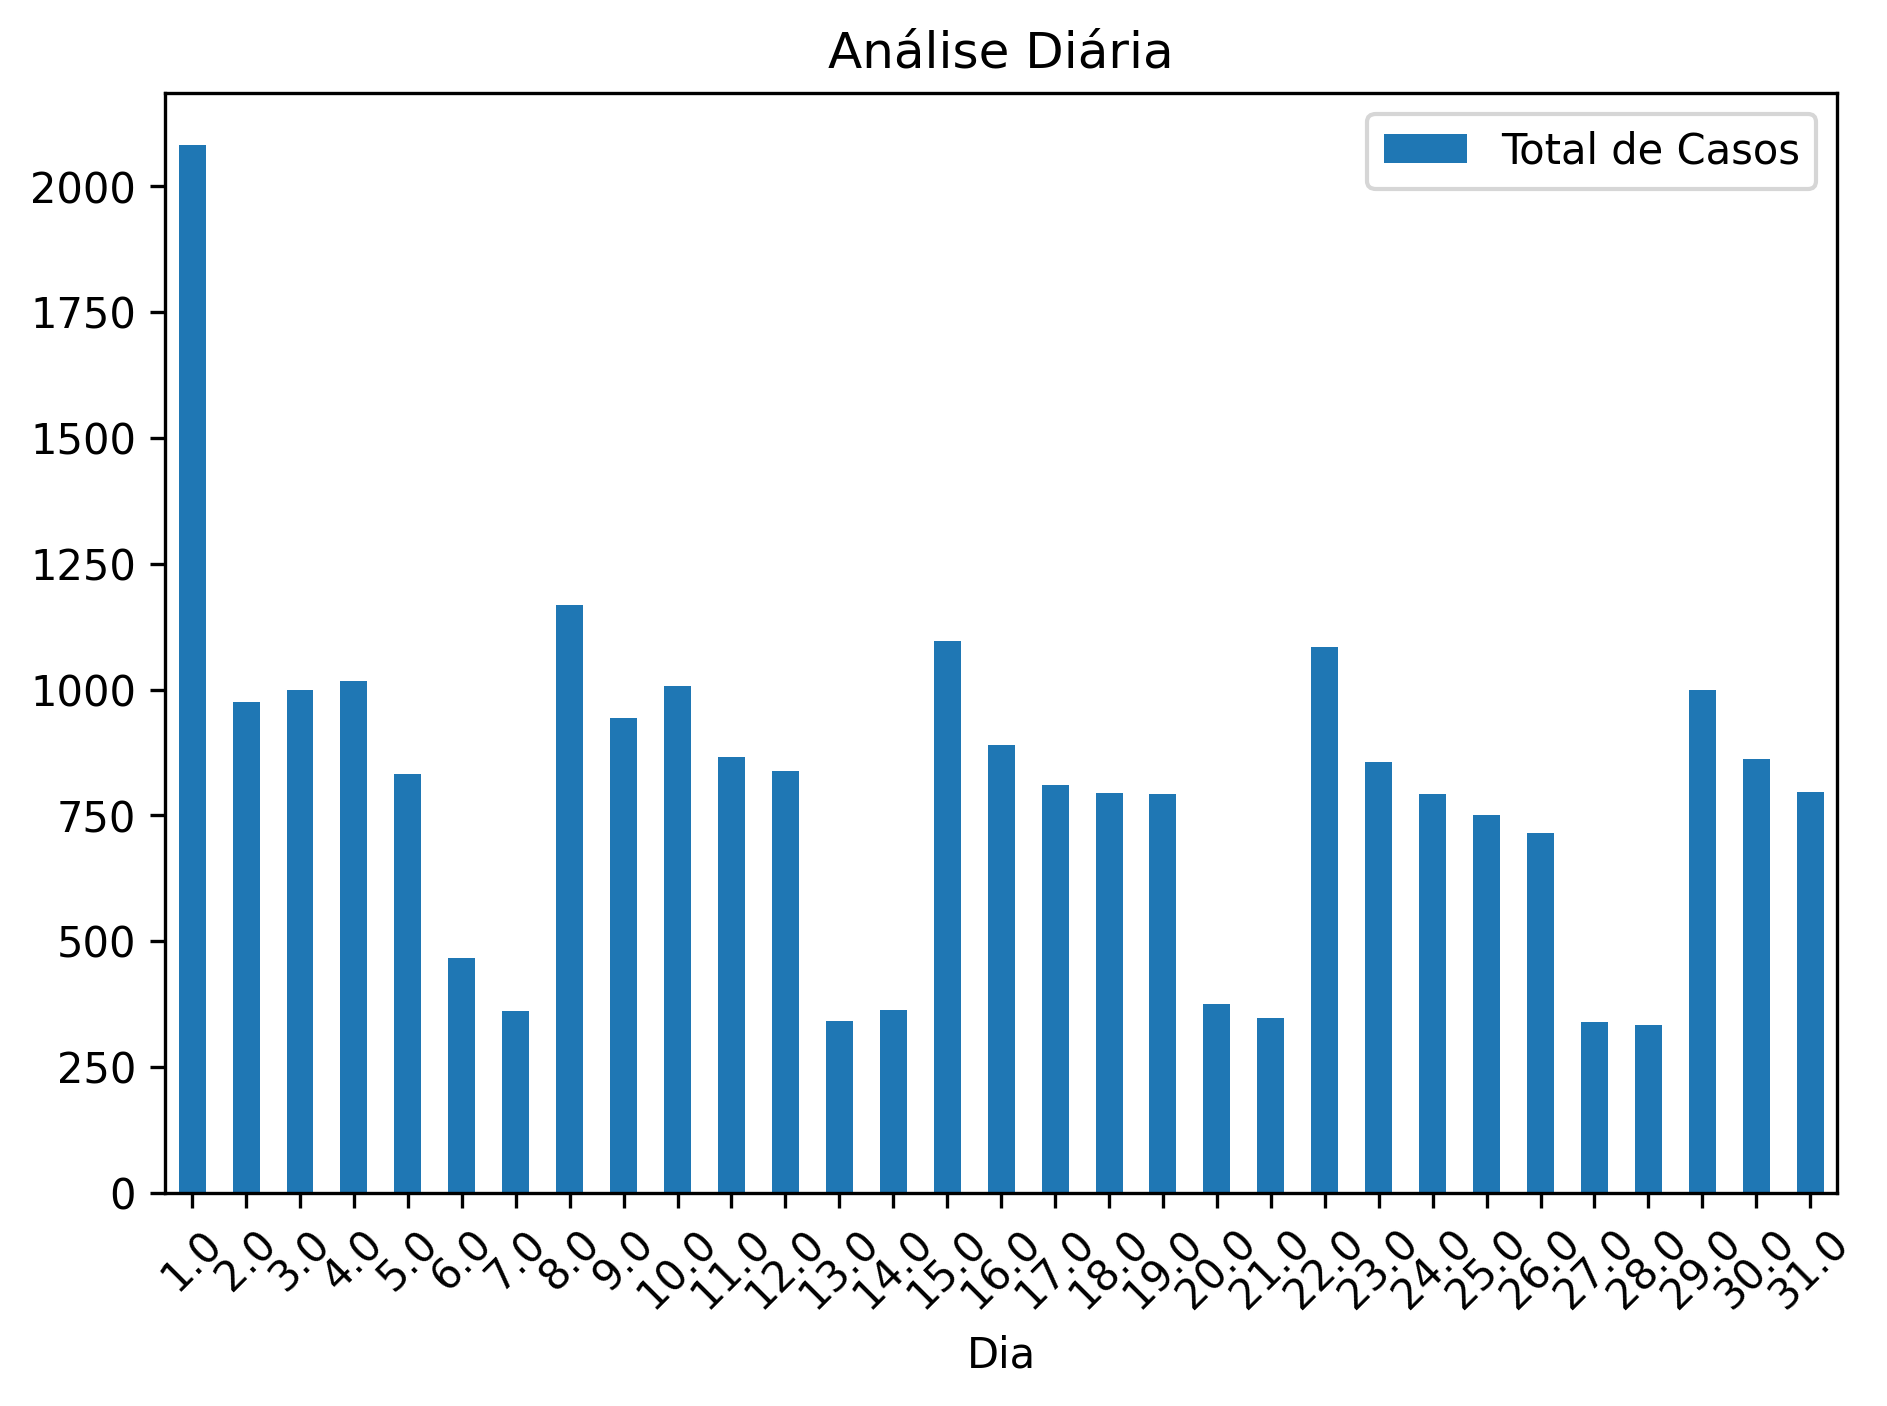
\includegraphics[width=\textwidth]{../graphics/monthly-analysis.png}%
\caption{Análise Mensal}%
\label{fig:casos-30-dias}%
\end{minipage}%
\begin{minipage}{0.45\textwidth}%
\centering%
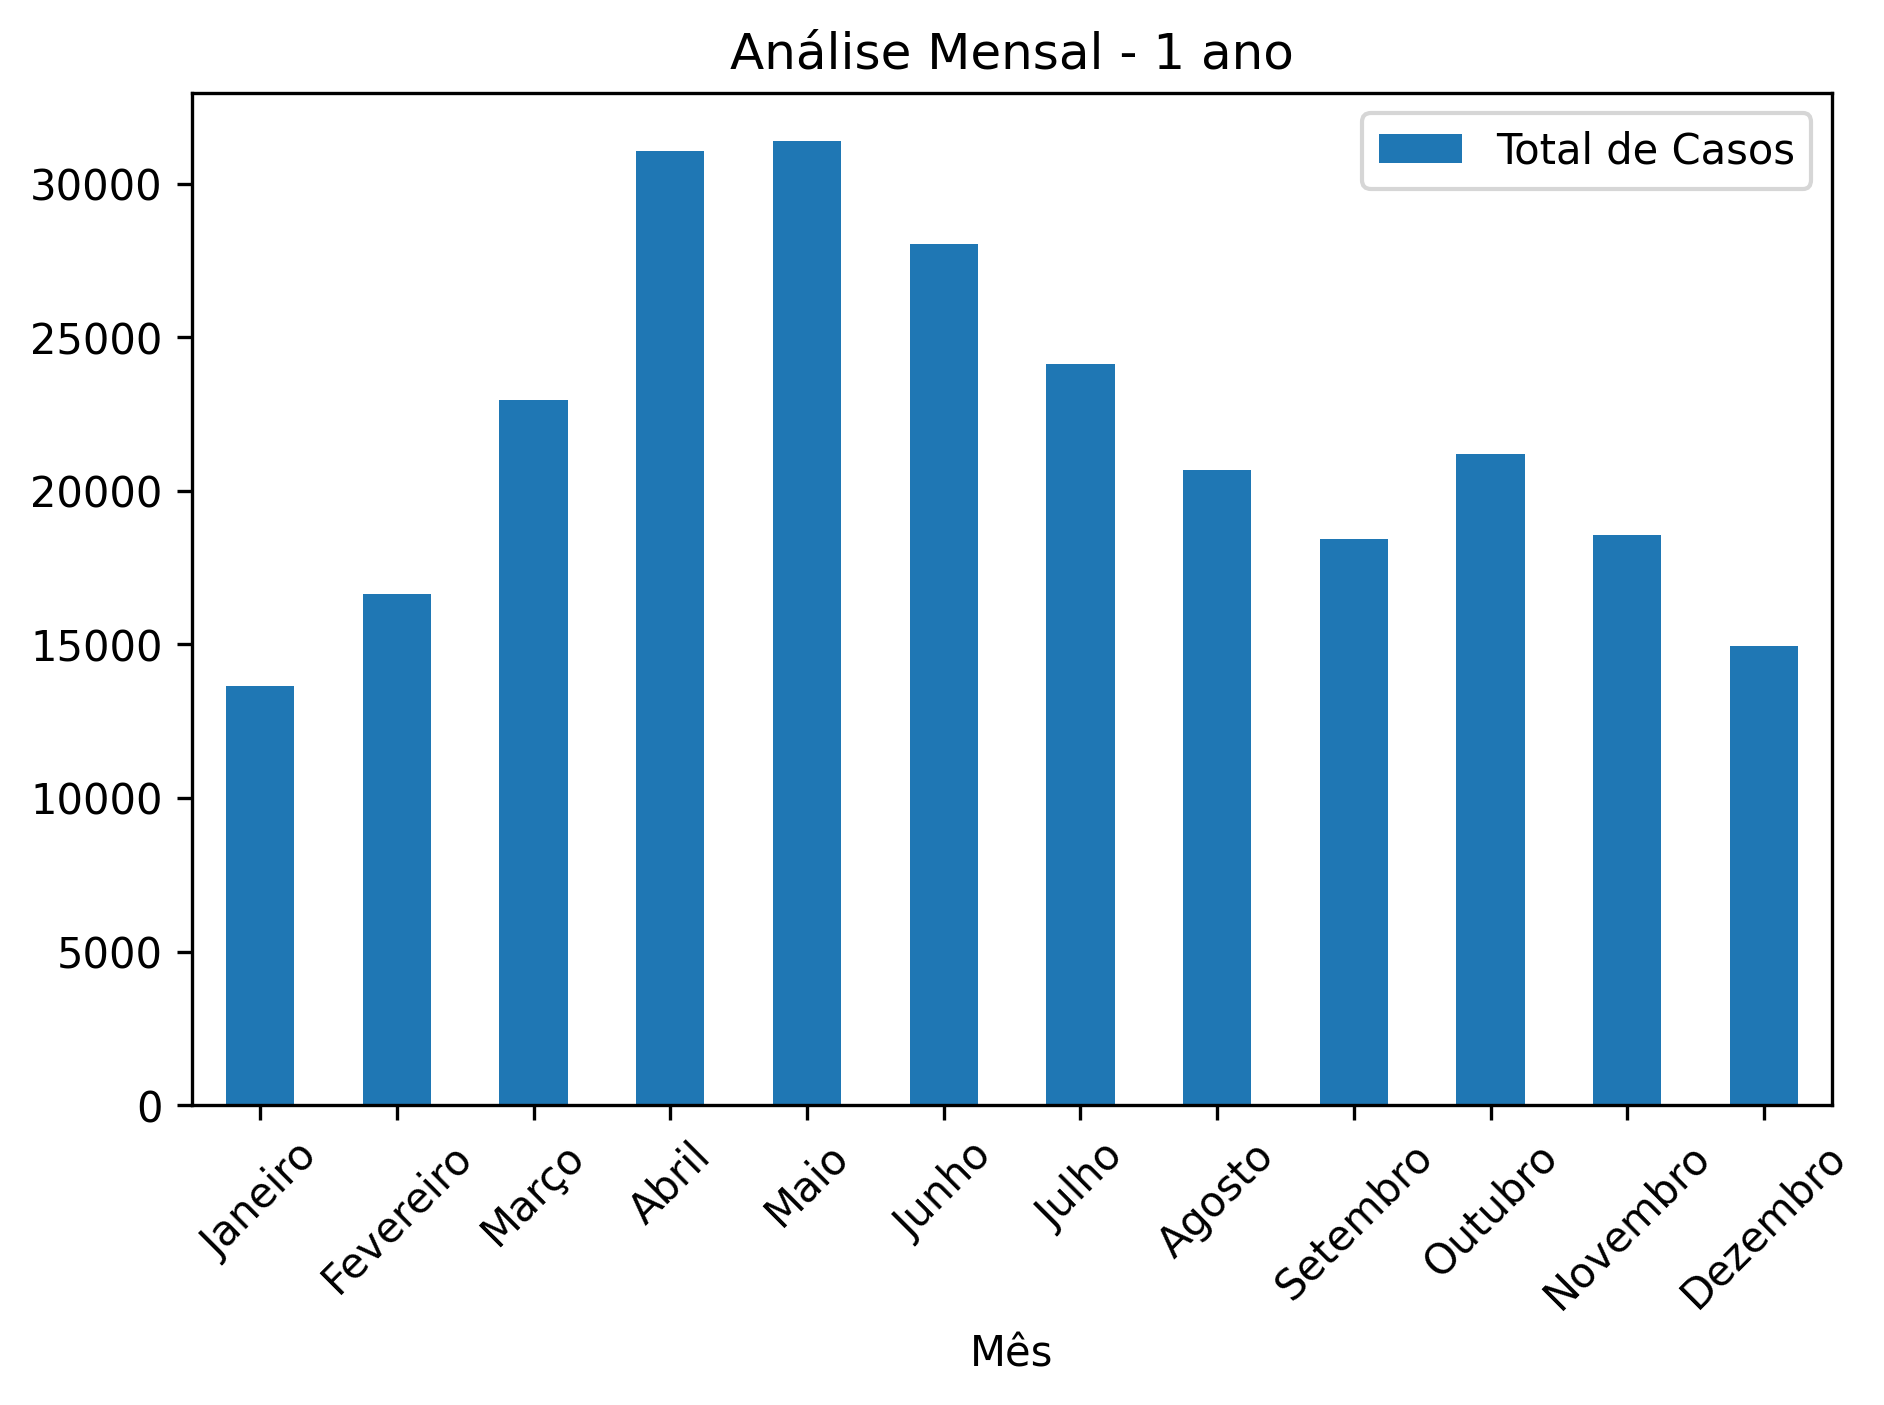
\includegraphics[width=\textwidth]{../graphics/yearly-analysis.png}%
\caption{Análise Anual}%
\label{fig:casos-12-meses}%
\end{minipage}%
\end{figure}

%
\end{document}